\documentclass[14pt,a4paper,oneside]{article}

\usepackage[utf8]{inputenc}   


\usepackage{amsmath,amsthm,amssymb,appendix,bm,mathrsfs,ctex,geometry,tcolorbox,fancyhdr,tikz,esint,appendix}


%% GB/T 7714 宏包 ---- 引文格式
\usepackage[sort&compress]{gbt7714}
\bibliographystyle{gbt7714-numerical}



\numberwithin{equation}{subsection}             %%%%%% 公式编号




\geometry{left=1.7cm, right=1.7cm, top=2.54cm, bottom=2.54cm}    %%%%% 页面尺寸
\linespread{1.5}                             %%%%% 行距1.5倍
\pagestyle{fancy}



%%    设置页眉页脚
\fancyhf{}
\renewcommand{\headrulewidth}{0.15mm}
\fancyhead[C]{文献阅读报告}                   %%%%%% 页眉
\fancyfoot[C]{\thepage}                      %%%%%% 页脚 页码
\setlength{\headheight}{15pt}


%%   设置各种链接颜色为黑色
\usepackage[colorlinks,
            linkcolor=black,
            anchorcolor=black,
            citecolor=black,
            urlcolor=black
            ]{hyperref}



%%   例子编号
\newcounter{example}
\counterwithin{example}{subsection}
\newcommand{\examplename}{Example}
\newcommand{\exampleTitle}[1]{%
\textbf{\refstepcounter{example}\examplename\theexample:#1}\par}


%%  插入图片配置
\usepackage{graphicx,subfigure}
\usepackage[]{caption2} %新增调用的宏包
\numberwithin{figure}{subsection}               %%%%%% 图片编号

\graphicspath{ {./Figure/} }            %%%%% 设置图片文件所在目录
\DeclareGraphicsExtensions{.pdf,.svg,.jpeg,.png,.jpg}     %%%%% 支持图片格式


%%    支持tikz作图
\usepackage{tikz}
\usetikzlibrary{backgrounds,arrows}


\usepackage{pgfplots}
\pgfplotsset{compat=1.15}
\usepackage{mathrsfs}


\title{\textbf{文献阅读报告 2\\Multi-pass cells for post-compression of ultrashort laser pulses}}                           %%%%% 标题
\author{骆禹天}                                           %%%%% 作者
\date{2024/**/**}                                        %%%%%% 日期

%%   定义一些数学格式
\newtheorem{theorem}{定理}[subsection]
\newtheorem{definition}[theorem]{定义}
\newtheorem{lemma}[theorem]{引理}
\newtheorem{corollary}[theorem]{推论}
\newtheorem{example}[theorem]{例}
\newtheorem{proposition}[theorem]{命题}
\renewcommand{\abstractname}{\Large\textbf{摘要}}




%-------------------- 开始文档  --------------------%



\begin{document}

\pagenumbering{Roman}         %%%%% 目录前页码统计按罗马数字

\maketitle

\setcounter{page}{1}          %%%%% 标题开始统计页数

%-------------------- 目录  --------------------%

\tableofcontents              %%%%% 插入目录

\newpage                      
\setcounter{page}{1}          %%%%% 目录后重新统计页数


\pagenumbering{arabic}        %%%%% 目录后统计页码为阿拉伯数字



%-------------------- 开始第一节  --------------------%



\section{Introduction}

超宽带钛宝石（Ti:Sa）激光器现逐渐被发射带宽较小但平均功率可扩展性更好的方案所取代，最突出的是掺镱（Yb）离子激光器。为实现由傅里叶变换极限所限制的，高功率激光的输出光谱的才具备的短脉冲持续时间（50fs以下），通常有两种途径：（1）超连续谱生成（OPCPA）；（2）光克尔效应实现光谱展宽。

基于Herriott型多通腔（MPC）的光谱增宽方法表现出巨大的优势：

（1）平均功率：第一篇研究MPC后压缩方法的论文发表于2016年，其展示了平均功率375 W的超快脉冲压缩。这一结果实现了相较固体芯(250 W)或空芯光子晶体光纤光谱展宽（HC-PCF, ≈100 W）更大，且与充气毛细管的记录(408 W)相当。\cite{schulteNonlinearPulseCompression2016}最近，MPC 技术已成为第一个且唯一能在平均功率 kW量级上实现将脉冲压缩至低于 50 fs的后压缩方法。\cite{grebingKilowattaveragepowerCompressionMillijoule2020}

（2）峰值功率：MPC补充了固体芯光纤和毛细管，缩短了5 MW和100 MW之间的空缺。该范围内的光谱增宽对高重复率掺Yb激光器产生能量在10 $\mathrm{\mu J}$到100 $\mathrm{\mu J}$量级的脉冲构成了重大挑战。\cite{schulteNonlinearPulseCompression2016}采用充气 MPC 可以将脉冲能量范围提高到 100 mJ 量级，\cite{kaumannsSpectralBroadening1122021}超过了毛细管实验的能量记录（40 mJ）并开启了产生峰值功率TW量级、重复频率kHz量级的超短脉冲的前景。

（3）高脉冲压缩因子：有报道将单级脉冲持续时间从1.2 ps减少到32 fs，最终持续时间进一步缩短到13 fs，实现了92的总压缩因子，\cite{ballaPostcompressionPicosecondPulses2020}证明了将高功率ps激光器变成少周期光源的原理。

（4）实用优势：（a）成本效低易实现；（b）鲁棒性良好，对波束指向非常不敏感，甚至可在无传输损耗情形处理小的模式失配\cite{vernalekenVerfahrenUndAnordung2017}。（c）结构紧凑，不需要大量系统长度的情况下获得大的B积分。

\section{用于光谱展宽的MPC}

\subsection{MPC概述}

MPC通常基于非线性介质（块材或气体）的自相位调制（SPM），SPM引起的啁啾随后被外部压缩器去除从而获得时间压缩的脉冲。或也可以采用自压缩，脉冲在光谱展宽阶段内被压缩。
	
最常用的Herriott型MPC由两个相同的凹面镜组成，如图 \ref{p2.1.1} 所示。类似于光学腔，Herriott单元形成横向本征模，并保留与MPC本征模匹配的光束模式的高斯光束q参数。Herriott腔增加了SPM的光路长度，每次光脉冲往返都会引入一个小的自相位调制，最终累积大的B积分获得带宽增益。MPC通过在非线性区域的重复传播以及利用腔镜适当地重新聚焦，从而实现大的展宽因子和光谱良好的空间均匀分布。

\begin{figure}[h]
    \centering
    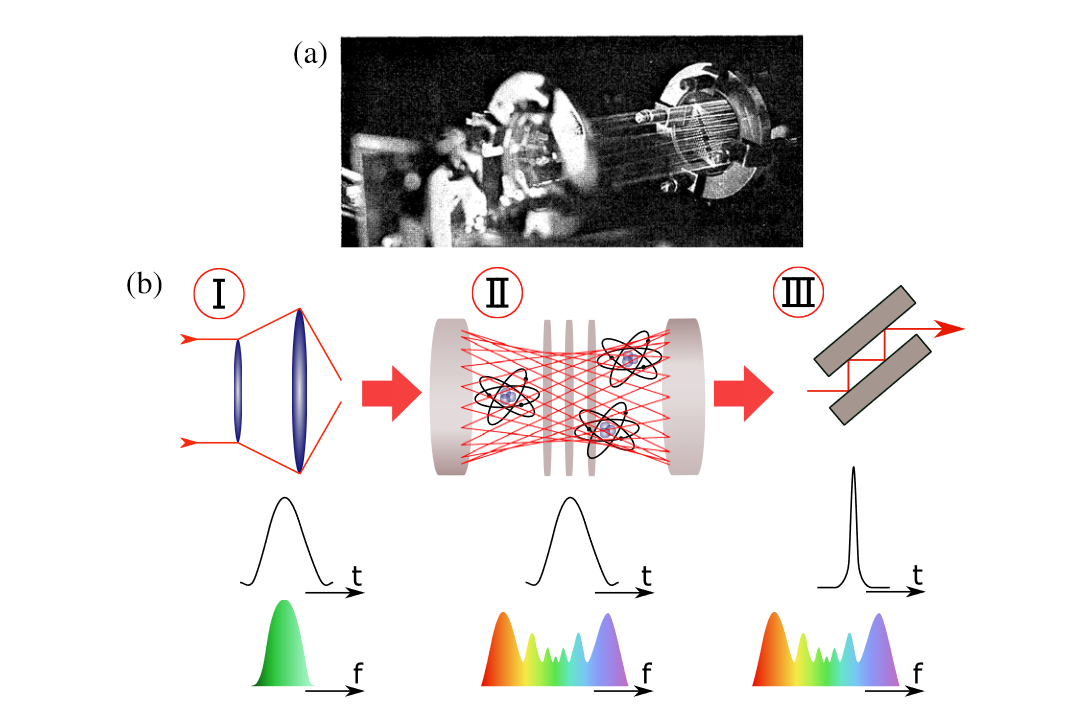
\includegraphics[width=0.4\columnwidth,height=0.3\linewidth]{p1.png}
    \caption{MPC结构原理示意图}\label{p2.1.1}
\end{figure}

MPC 结构如图 \ref{p2.1.1} 所示，激光光束先通过一个望远镜结构 (I) 调节与 MPC 的本征模式进行模式匹配，从而确保每次穿过腔镜时具有相同的光束属性。随后，光束通过耦合镜耦合进 MPC (II) 中。达到目标通数后，输出光束通过另一个耦合镜耦合出去。最后需要对光束进行准直，并且通过光栅对压缩器或啁啾镜压缩器 (III) 来消除啁啾将脉冲压缩至接近变换极限。

\subsection{Herriott 型 MPC 关键参数}

\subsubsection{MPC 光斑分布与再入条件}

1964 年，Herriott、Kogelnik 和 Kompfner研究了两个相对的凹面镜组成腔体的光斑图案，这样的凸面镜等效为一系列等距薄透镜，如图\ref{p2.2.1}(a)。光学系统的周期性导致在 0 < L < 2R 稳定范围内每次往返后，光斑的横向位置坐标 x 和 y 正弦增加，其中 L 是反射镜距离，R 是曲率半径。这对应光斑相对腔镜中心旋转了一个角度 $\xi$，如图\ref{p2.2.1}(b)。

\begin{figure}[h]
    \centering
    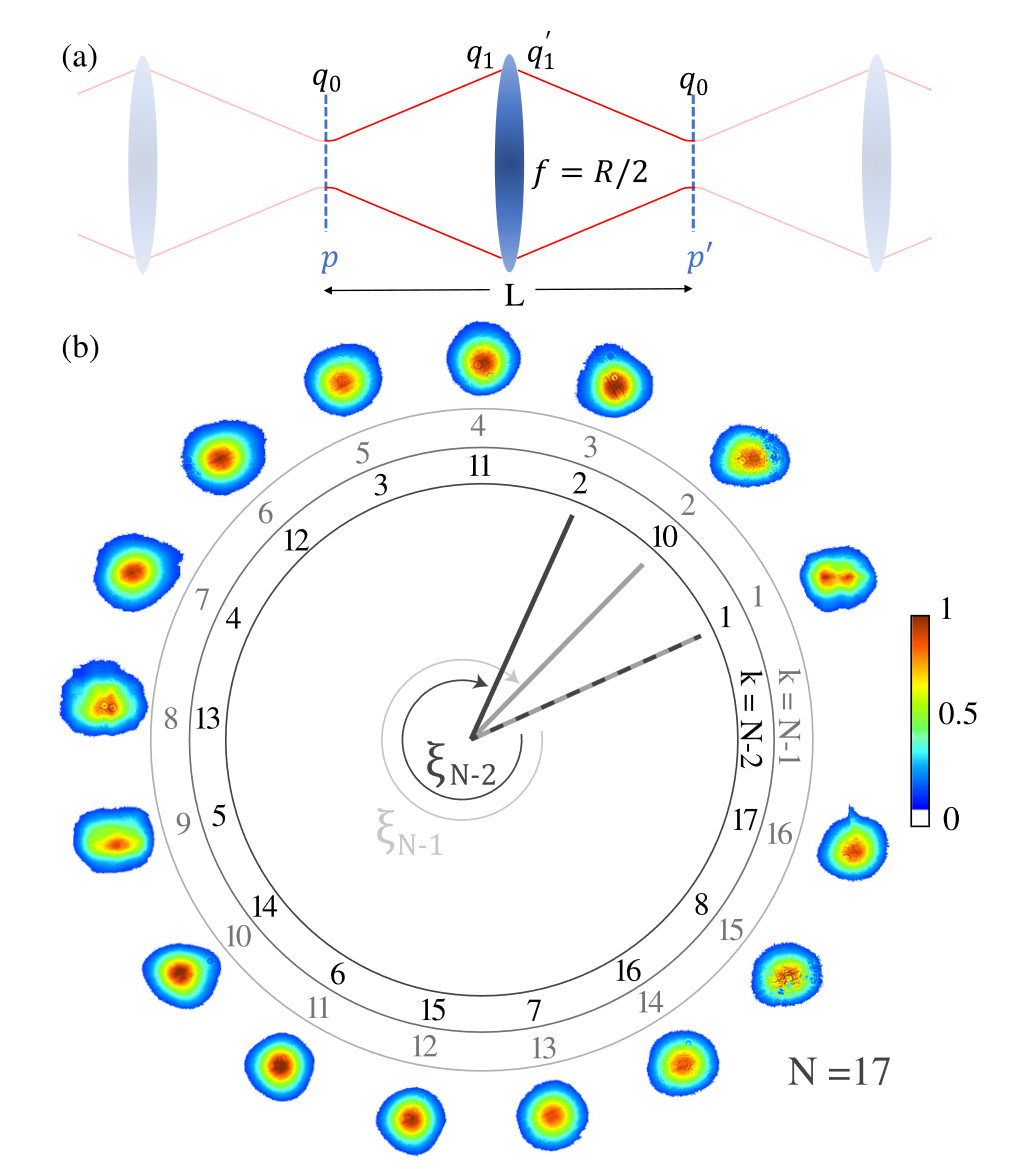
\includegraphics[width=0.5\columnwidth,height=0.6\linewidth]{p2.png}
    \caption{（a） Herriott腔等效于透镜周期序列。模式匹配下，q参数在边界处是常数（在p，p′处，$q=q_0$）。（b） 在k=N−1情况下，在MPC反射镜处测量的光束模式。}
    \label{p2.2.1}
\end{figure}

如果光在 N 次往返后耦合进和出腔体于同一位置，即满足再入条件，则该角度总和应为 2$\pi$ 的整数倍：
\begin{equation}
    \xi=2\pi k/N,\quad\mathrm{where\quad }k=1,\ldots,N-1
    \label{eq:2.2.1}
\end{equation}

因此，对于给定的腔镜半径R和旋转周期数N，可以由下式确定腔体长度L：
\begin{equation}
    C=\frac LR=1-\cos(\xi/2)=1-\cos(\pi k/N) 
    \label{eq:2.2.2}
\end{equation}

\subsubsection{MPC模式匹配}

可利用图\ref{p2.2.1}（a）中的等效透镜波导推导具有高斯横向本征模的两个镜面光学谐振器的稳定性条件。腔体内的镜像对称性要求，薄透镜必须反转光束的曲率，使光束的曲率半径保持为R。使用ABCD矩阵来计算由高斯光束参数 $q_0$ 表示的横向高斯本征模。从图\ref{p2.2.1}（a）中，L/2和反射镜的传播矩阵可以组合为
\begin{equation}
    \begin{aligned}M^j&=(M_{\mathrm{prop}}\cdot M_{\mathrm{mirror}}\cdot M_{\mathrm{prop}})^j\\&=\begin{bmatrix}1-C&RC(1-C/2)\\-2/R&1-C\end{bmatrix}^j\end{aligned}
    \label{eq:2.2.3}
\end{equation}
其中，C＝L/R。对于任意整数j，$q_0$应有相同的值。令j=1，有：
\begin{equation}
    q_0=\frac{(1-C)q_0+RC(1-C/2)}{(-2/R)q_0+1-C}
    \label{eq:2.2.4}
\end{equation}
解得：
\begin{equation}
    q_0=-\frac R2\sqrt{C(C-2)}
    \label{eq:2.2.5}
\end{equation}
可计算瑞利长度：
\begin{equation}
    z_R=-iq_0=\frac R2\sqrt{C(2-C)}
    \label{eq:2.2.6}
\end{equation}
由此可得聚焦和反射镜处的光束的半径：
\begin{equation}
    w_0^2=\frac{R\lambda}{2\pi}\sqrt{C(2-C)}=\frac{R\lambda}{2\pi}\sin(\pi k/N)\overset{k/N\to1}{\operatorname*{\approx}}\frac{R\lambda}{2N}
    \label{eq:2.2.7}
\end{equation}
\begin{equation}
    w_m^2=\frac{R\lambda}\pi\sqrt{\frac C{2-C}}=\frac{R\lambda}\pi\tan(\pi k/2N)\overset{k/N\to1}{\operatorname*{\approx}}\frac{2R\lambda N}{\pi^2}
    \label{eq:2.2.8}
\end{equation}

通常限制MPC的最大脉冲能量的两个相关量是MPC反射镜的激光诱导损伤阈值（LIDT），通常通过通量$F_m$以及聚焦峰值强度$I_0$来量化，其可以计算为：
\begin{equation}
    F_m=\frac{2E}{R\lambda}\sqrt{\frac{2-C}C}=\frac{2E}{R\lambda}\frac1{\tan(\pi k/2N)}\overset{k/N\to1}{\operatorname*{\approx}}\frac{\pi E}{R\lambda N}
    \label{eq:2.2.9}
\end{equation}
\begin{equation}
    I_0=\frac{4P}{R\lambda}\frac1{\sqrt{C(2-C)}}=\frac{4P}{R\lambda}\frac1{\sin(\pi k/N)}\overset{k/N\to1}{\operatorname*{\approx}}\frac{4PN}{\pi R\lambda}
    \label{eq:2.2.10}
\end{equation}
这里，E和P分别是脉冲能量和脉冲峰值功率。

上述方程忽略了Herriott腔内的自聚焦。实际中，自聚焦会在光谱展宽过程中改变光斑尺寸，其影响应在模式匹配中加以考虑。尤其$F_m$和$I_0$可能明显大于由等式\ref{eq:2.2.9}和\ref{eq:2.2.10}得到的值。在充气MPC中，额外的自聚焦有效地减少了光束发散，从而在反射镜和束腰处产生较小的光斑尺寸，用于非线性模式匹配。固体MPC通常在Kerr透镜更强的临界自聚焦状态下进行。这可能会引入单通内额外的弱的引导效果。

Q：文献图\ref{p2.2.1}中，$f=R/2$，是否应当使用厚透镜公式？
\begin{equation}
    \frac{1}{f}=(n-1)\left[\frac{1}{R_1}-\frac{1}{R_2}+\frac{(n-1)d}{nR_1R_2}\right]
    \label{eq:2.2.3}
\end{equation}

\subsubsection{MPC光谱展宽}

为了量化光谱展宽，常使用B积分进行衡量。这里，我们将B积分定义为轴上累积的非线性相位，即：
\begin{equation}
    B:=\frac{2\pi}{\lambda} \int n_2I_p(z)\mathrm{d}z
    \label{eq:2.2.11}
\end{equation}
其中，$I_p(z)$表示光轴z上的峰值强度，$n_2$表示介质非线性折射率。也有其他论文中，B积分等于最大非线性相移
\begin{equation}
    \phi_{max}:=\frac{2π}{\lambda}\int \frac{n_2P}{A_{\mathrm{eff}}}\mathrm{d}z
    \label{eq:2.2.12}
\end{equation}
其中，$A_{\mathrm{eff}}$是有效模面积。通常这两个数量并不相同。对高斯光束$B=2\phi_{\mathrm{max}}$在对称MPC内的无损耗和无色散传播，单通B积分为
\begin{equation}
    B_{\mathrm{pass}}=2\phi_{\mathrm{max,pass}}=4\pi\frac{n_2P}{\lambda^2z_R}\int_{d_k}^{d_K+l_K}(1+\frac{z^2}{z_R^2})^{-1}\mathrm{d}z
    \label{eq:2.2.13}
\end{equation}
这里，$d_K$是从腔中心到克尔介质的距离，$l_K$是克尔介质的长度，$z_R$是瑞利长度。对于均匀非线性介质的MPC，可用$\frac{R}{2\sqrt{C(2−C)}}$代入瑞利长度$z_R$，方程 \ref{eq:2.2.13}简化为
\begin{equation}
    B_{\mathrm{pass}}=4\pi^2\frac{n_2P}{\lambda^2}\frac kN\leq\frac{2\pi k}{N}
    \label{eq:2.2.14}
\end{equation}
每次通过MPC的B积分受自聚焦功率阈值的限制，等号对应功率达到自聚焦功率阈值的情形。
\begin{equation}
    P=P_{\mathrm{crit}}≈\frac{\lambda^2}{2πn_0n_2}
    \label{eq:2.2.15}
\end{equation}
此时，方程\ref{eq:2.2.14}在$n_0=1$和$k/N\rightarrow 1$时给出
\begin{equation}
    B_{pass,c}=\frac{2\pi k}{N}\approx 2\pi
    \label{eq:2.2.16}
\end{equation}
方程\ref{eq:2.2.14}表明，B积分不依赖于MPC的尺寸。然而，最大B积分即最大光谱展宽随k减小，如图 \ref{p2.2.2} (b)所示。在固体MPC中，单通的B积分通常较小，充气MPC则大得多。然而，若将多个二氧化硅薄板插入MPC中，可产生与充气MPC相当的单通B积分$\approx0.8\pi$。

\begin{figure}[h]
    \centering
    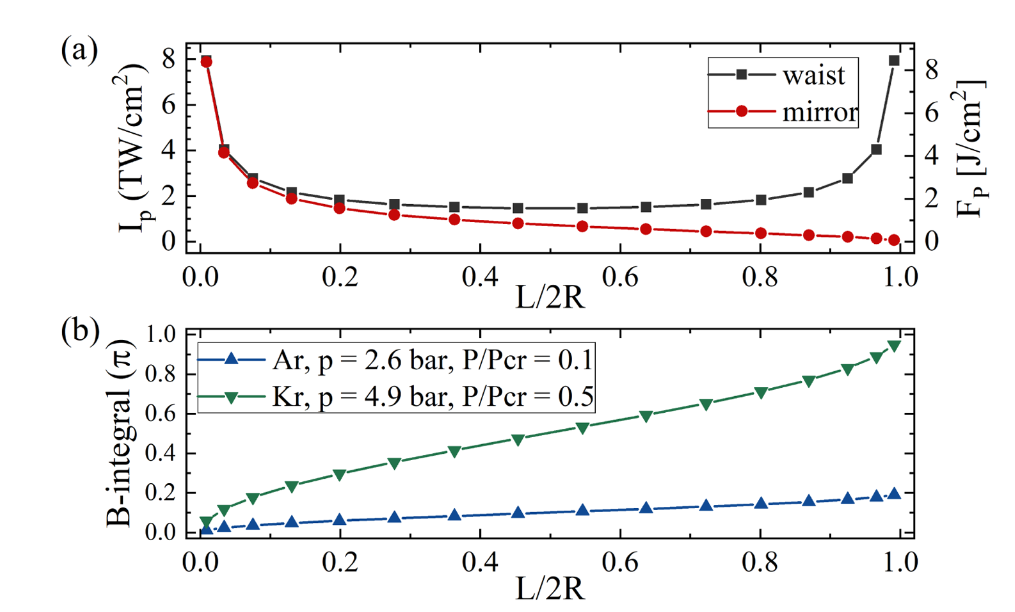
\includegraphics[width=0.6\columnwidth,height=0.4\linewidth]{p3.png}
    \caption{（a）在腔中心和MPC反射镜处计算的峰值强度$I_p$和峰值通量$F_p$；（b）不同的气体和压力，每通的B积分}
    \label{p2.2.2}
\end{figure}

有一种非常简单的方法可以用来估计光谱展宽因子。将式 \ref{eq:2.2.10} 代入式\ref{eq:2.2.11}，有均匀非线性介质MPC中，傍轴高斯光束每次通过的B积分为：
\begin{equation}
        B_{\mathrm{pass}}=\int_{x=-L/2}^{+L/2}\frac{2\pi n_2}\lambda I(z)\mathrm{d}z=\frac{8\pi}{\lambda^2}Pn_2\mathrm{tan}^{-1}\left(\sqrt{\frac C{2-C}}\right)
    \label{eq:2.2.17}
\end{equation}

若代入 $C=1-\cos(\frac{\pi k}{N})=2\sin^2(\frac{\pi k}{2N})$，
\begin{equation}
    B_{\mathrm{pass}}=4\pi^2\frac{Pn_2}{\lambda^2}\frac kN
    \label{eq:2.2.18}
\end{equation}
得到与式\ref{eq:2.2.14}结果一致。

由于高斯脉冲的光谱展宽因子为
\begin{equation}
    b=\frac{\Delta\omega}{\Delta\omega_0}=\sqrt{1+\frac4{3\sqrt{3}}\phi_{\max}^2},
    \label{eq:2.2.19}
\end{equation}
对于较大的 $\phi_{\mathrm{max}}$，约有比例： $b\approx 0.88\phi_{\mathrm{max}}$。代入式\ref{eq:2.2.17}，由于高斯光束的 $B=2\phi_{\mathrm{max}}$，我们有MPC的光谱增宽为（考虑N次往返，亦即2N次通过非线性介质）：
\begin{equation}
    b=\sqrt{1+\frac4{3\sqrt{3}}{\left(2N\times\frac{8\pi}{\lambda^2}Pn_2{\tan}^{-1}\left(\sqrt{\frac C{2-C}}\right)\right)^2}}
    \label{eq:2.2.20}
\end{equation}
对于大的B和C $\rightarrow 2$，平方根中第一项可忽略，正切函数反函数项接近 $\pi/2$。最后，结果如下：
\begin{equation}
    b=\frac{\Delta\omega_{\mathrm{out}}}{\Delta\omega_{\mathrm{in}}}=\sqrt{1+\frac4{3\sqrt{3}}\phi_{\mathrm{max}^2}^2}\approx0.88\phi_{\mathrm{max}}
    \label{eq:2.2.21}
\end{equation}
\begin{equation}
    \approx7\pi^2\frac{n_2Pk}{2\lambda^2}\overset{N\to1}{\operatorname*{\approx}}7\pi^2\frac{n_2PN}{2\lambda^2}\quad\quad\quad\quad\quad\quad
    \label{eq:2.2.22}
\end{equation}


这里，我们假设了脉冲形状为为时域下变换极限的高斯脉冲并且假设由于诸如色散等因素引起的时间脉冲整形的影响可以忽略。

时间压缩比$K$定义为输入脉冲的半峰全宽（FWHM）与压缩脉冲间的比值。考虑初始高斯脉冲和由此产生的SPM展宽后的变换极限脉冲，我们有：
\begin{equation}
    K\approx0.59\phi_{\max}+1\overset{B\gg1}{\operatorname*{\approx}}B/\pi \quad
    \label{eq:2.2.23}
\end{equation}
\begin{equation}
    \approx8\pi\frac{n_2Pk}{\lambda^2}\overset{N\to1}{\operatorname*{\approx}}8\pi\frac{n_2PN}{\lambda^2}
    \label{eq:2.2.24}
\end{equation}

注意：式\ref{eq:2.2.21}和\ref{eq:2.2.23}通常成立，且可在光学克尔效应占主导时使用，而式\ref{eq:2.2.22}和\ref{eq:2.2.24}仅适用于充满均匀非线性介质的MPC。

\subsubsection{MPC设计}

我们将讨论配置MPC时需要考虑的几个基本步骤。这里只考虑具有圆形光束图案的对称Herriott型MPC，使用气体或固体作为非线性介质。表1中展示了文献中的几个MPC示例的参数。


\begin{table}[!ht]
    \renewcommand{\arraystretch}{2}
	\centering\fontsize{6pt}{2}\selectfont
    \caption{MPC示例}
    \begin{tabular}{ccccccccccccc}
    \hline
    Medium&$n_2$($cm^2/W$) &$l_k$ (mm) &p (bar) &L (mm) &R (mm) &k &N &P (MW) &$F_m$ ($mJ/cm^2$) &$I_0$ ($GW/cm^2$) &B ($\pi$ ) &$K_{\mathrm{exp}}$\\\hline
    FS &$2.8 \times 10^{-16}$ &$2 \times 13$ &N/A &540 &350 &13 &19 &46 &11 &14 & 6.7 & 5 \\
    FS &$2.8 \times 10^{-16}$ &25 &N/A &500 &300 &41 &55.5 &16 &30 &14 &18.2 &20.8 \\
    FS &$2.8 \times 10^{-16}$ &$6 \times 1$ &N/A &385 &200 &28 &32 &85 &20 &$0.4 \times 10^3$ &53.7 &32 \\
    Ar &$4.2 \times 10^{-20}$ &N/A &0.6 &2985 &1500 &22 &22.5 &$13 \times 10^3$ &155 &$22 \times 10^3$ &25.4 &32 \\
    Ar &$2.4 \times 10^{-19}$ &N/A &3.5 &788 &400 &27 &29 &$1.7 \times 10^3$ &58 &$6.1 \times 10^3$ &23.1 &22.3 \\
    Ar &$4.9 \times 10^{-19}$ &N/A &7 &286.5 &300 &17 &34 &550 &94 &$0.6 \times 10^3$ &8.8 &8.3\\
    \hline
    \end{tabular}
\end{table}

• 非线性介质：

（1）气体（惰性气体）；

（2）：固体（涂有抗反射镀层的熔融石英）。

• 腔镜：

（1）曲率通常接近腔长，保证足够低的反射镜通量和聚焦峰值强度以避免损伤或电离;

（2）商用非色散介质镜的激光诱导损伤阈值（光学器件推测的损伤概率为零的最高激光辐射量，LIDT）约为1 $\mathrm{J/cm^2}$，脉冲持续时间为1 ps。注意，LIDT相关于许多激光参数，包括光束尺寸，一般将通量限制在LIDT$\leq2$以下，可为安全操作留出足够的空间；

（3）对确定的配置参数k，N，腔长不影响填充有均匀非线性介质的MPC的光谱展宽因子[参见等式\ref{eq:2.2.22}]。

• k、N：对固定的反射镜曲率半径，k和N仅通过微调MPC长度来选择。N的选择主要取决于目标压缩因子[式 \ref{eq:2.2.23}和 \ref{eq:2.2.24}]。N的典型值在15到30范围内。更大的N能产生更大的压缩比，但应避免k/N=1，k/N=1对应于4f成像情形，会使光束质量变差。充气MPC的典型选择是k=N−1，这种配置下光谱增展宽因子最大，同时反射镜处的光通量最小。对于固体MPC，在不增加系统长度的情况下，在k＜N−1的条件下操作可能能够增加通数，从而实现更大展宽。

• 反射镜直径由通数决定，因为它决定了圆形图案中相邻点间的最大距离。而为确保输入或输出耦合的损失最小需要足够的距离。

• 应选择镜面涂层以支持足够反射率。标准四分之一波片反射镜可提供足够光谱宽度以支持约30 fs的脉冲，同时保持低色散。在1030 nm左右，MPC反射镜最常见的层排列是Ta2O5/SiO2或HfO2/SiO2堆叠，其中HfO2/SiO2堆叠能够提供最大的损伤阈值。通过使用较低带隙的高折射率材料，例如TiO2/SiO2堆叠，可以获得稍短的脉冲，但较低的带隙也导致较低的损伤阈值。当甚至需要更大的带宽时，例如，对于几个周期的脉冲生成，则很容易达到标准电介质涂层的带宽极限。

•压缩器：MPC光谱增宽获得的啁啾量很小，类似于光纤，通常使用光栅对或啁啾镜压缩器。

\subsubsection{MPC 的数值模拟}

如前文所述，空腔几何形状规定了MPC模式，可以通过简单的ABCD矩阵来计算最基本的腔体参数。

为了评估基于MPC的后压缩系统中非线性效应对光脉冲的影响，通常采用脉冲传播的3D数值模型。

Hanna等人使用基于对称分步傅立叶算法的3D模型来研究时空耦合，该算法适用于充气和散装MPC\cite{hannaNonlinearTemporalCompression2017}。随后，提出了一种能够预测MPC中时间和光谱传播的简化1D模型，该模型、3D模型和实验的结果相互一致，验证了1D模型的合理性，大大减少计算时间。\cite{daherMultipassCells1D2020}

更一般地，用于非线性脉冲传播的标准方法可以容易地适用于MPC。Couairon等人完整介绍了非线性介质中超短脉冲传播建模的数值方法\cite{couaironPractitionerGuideLaser}。

G.Arisholm开发的SISYFOS代码使用傅立叶空间方法来求解传播方程，并且可以处理MPC中的宽带宽[54]。

也可以使用一些开源模拟包，例如Python包PyNLO\cite{barbieroEfficientNonlinearCompression2021}。MPC数值模拟方法的更技术概述可以在最近的一篇综述文章中找到\cite{hannaNonlinearOpticsMultipass2021}。





%--------------------  附录  --------------------%



\newpage
\appendix
\appendixpage
\addappheadtotoc
\renewcommand{\appendixname}{Appendix~\Alph{section}}

\numberwithin{equation}{section}             %%%%%% 公式编号
\numberwithin{figure}{section}            %%%%%% 图片编号

\section{高斯光束q参数的变化规律}
沿z方向传播的基膜高斯光束场可表示为如下形式
\begin{equation}
    \phi_{00}(x,y,z)=\frac{c}{\omega(z)}e^{-i\frac{r^2}{\omega^2(z)}}e^{-i[k(z+\frac{r^2}{2R}-\arctan\frac{z}{f})]}
    \label{eq:A.1}
\end{equation}
其中，高斯光束有如下参数：
\begin{equation}
    \left\{\quad 
    \begin{aligned}
    &r^2=x^2=y^2\\
    &k=\frac{2\pi}{\lambda}\\
    &\omega(z)=\omega_0\sqrt{1+(\frac{z}{f})^2}\\
    &R(z)=z[1+   \left(\frac{f}{z}\right)^2]=z[1+(\frac{\pi\omega_0^2}{\lambda z})^2]\\
    &f=\frac{\pi\omega_0^2}{\lambda},\omega_0=\sqrt{\frac{\lambda f}{\pi}}
    \end{aligned}\right.
    \label{eq:A.2}
\end{equation}

$\omega_0$：基膜高斯光束的腰斑半径；

f：高斯光束的共焦参数；

R(z)：与传播轴线相交于z点的高斯光束等相面曲率半径；

$\omega(z)$：与传播轴线相交于z点的高斯光束等相面上的光斑半径。

\begin{figure}[h]
    \centering
    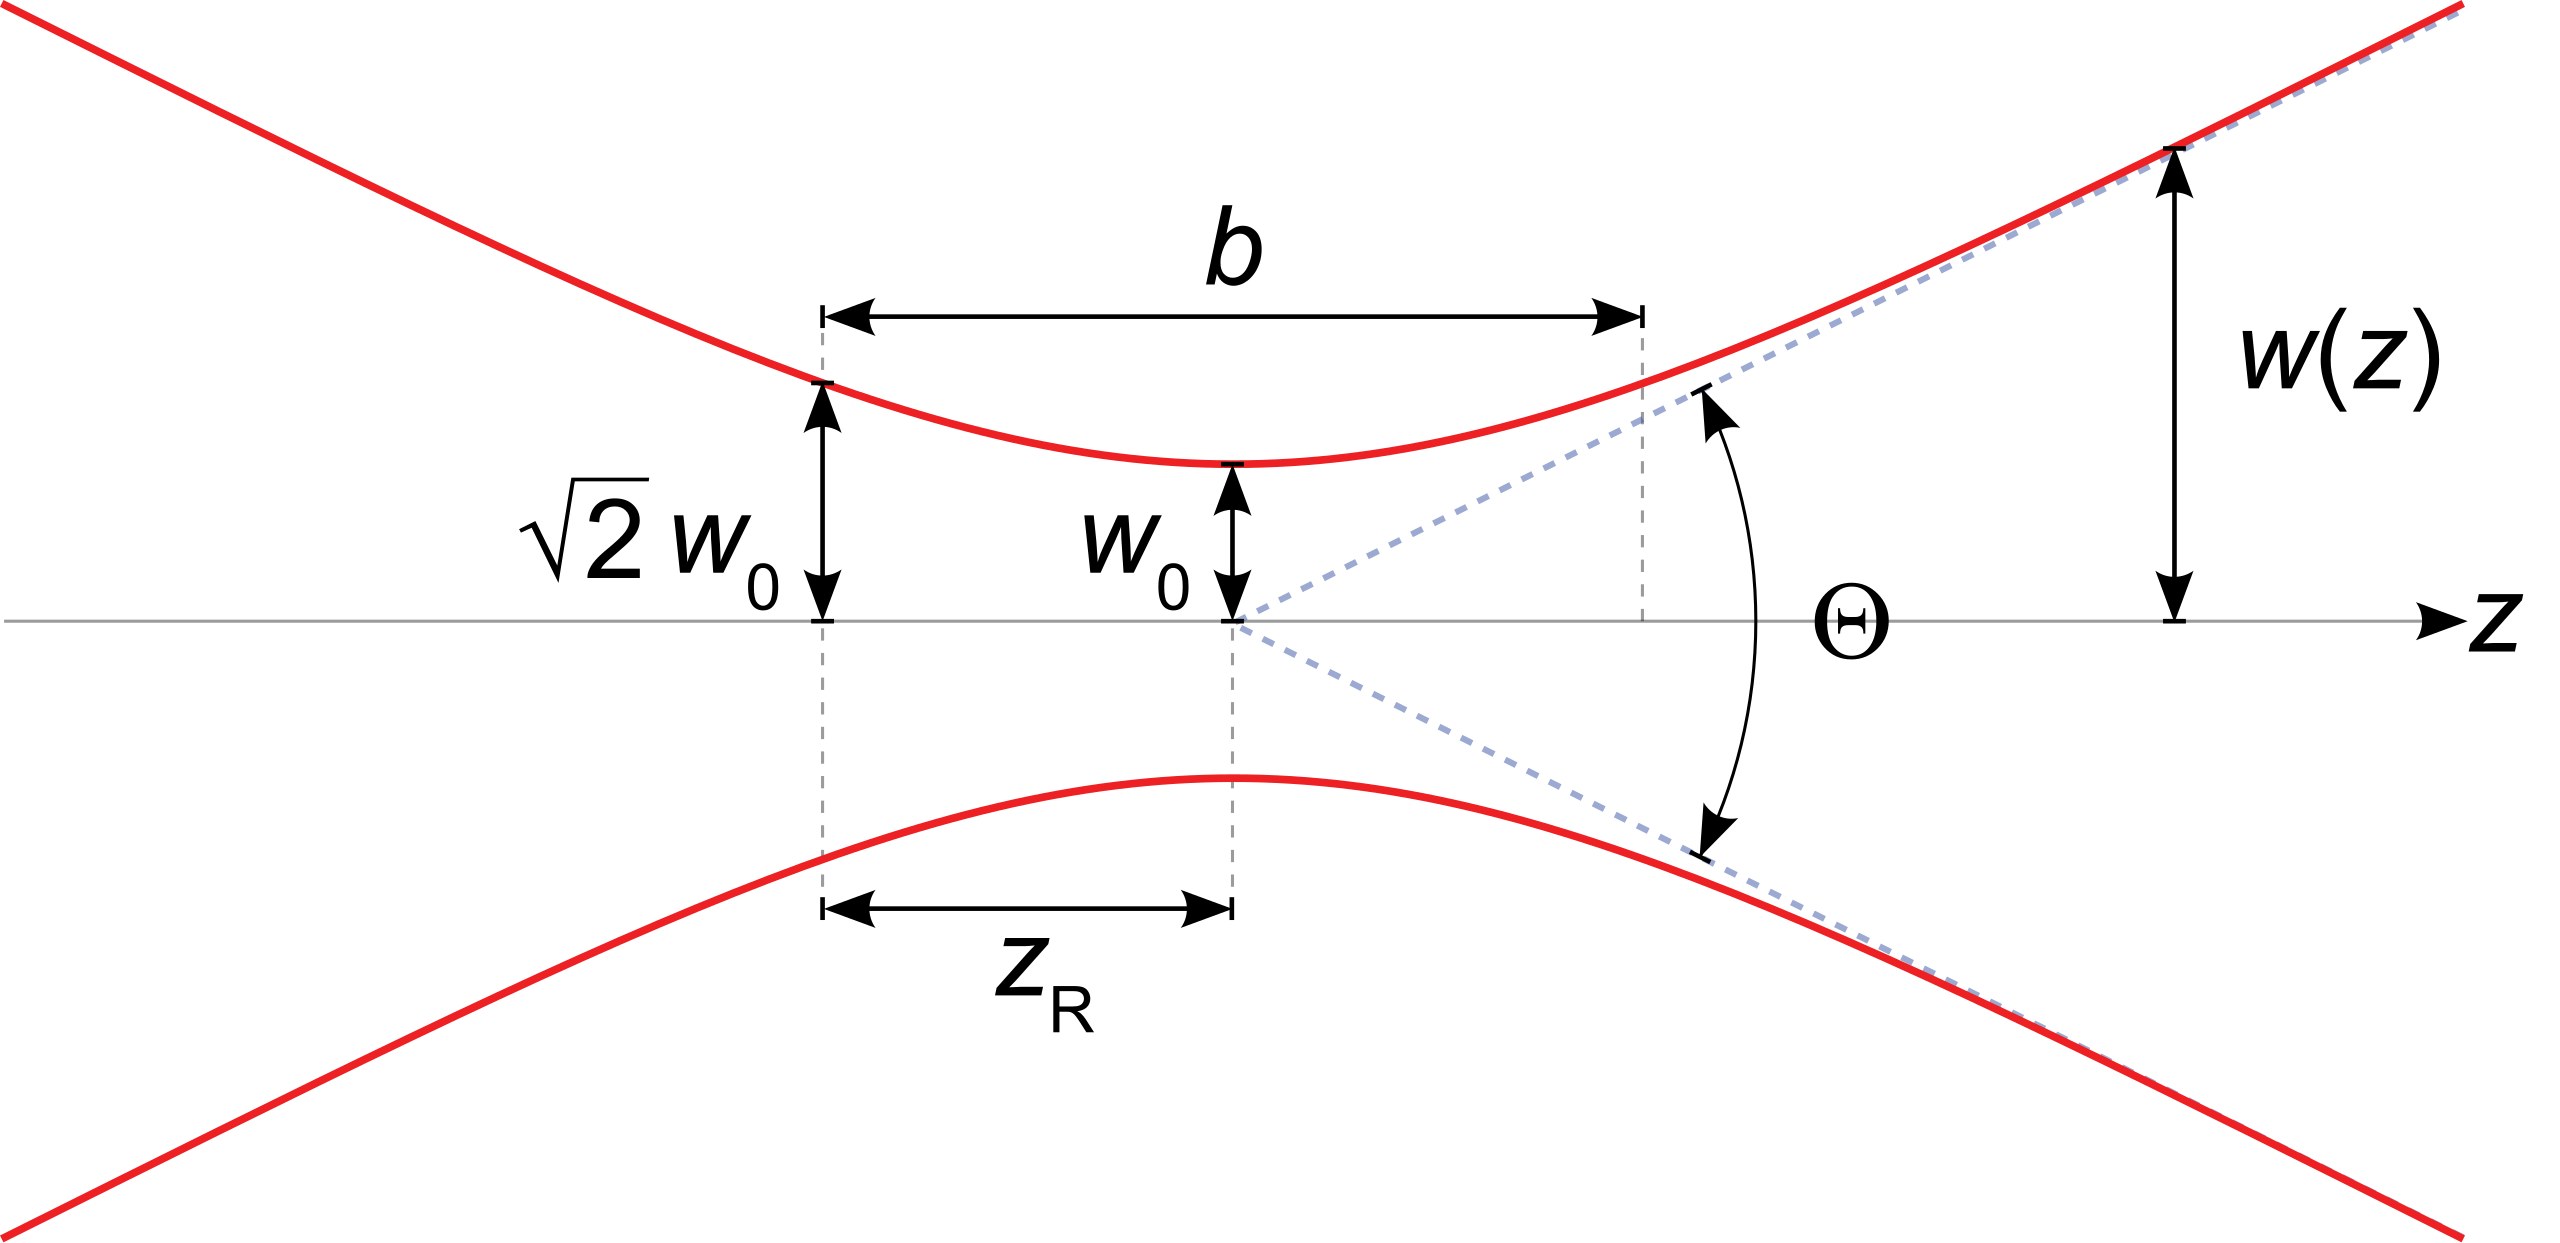
\includegraphics[width=0.35\textwidth]{appendix p1.png}
    \caption{高斯光束}\label{pA.1}
\end{figure}

q参数定义：
\begin{equation}
    \frac{1}{q(z)} =\frac{1}{R(z)}-i\frac{\lambda}{\pi\omega^2(z)} 
    \label{eq:A.3}
\end{equation}

代入R(z)和 $\omega(z)$
\begin{equation}
    \begin{aligned}
    &R(z)=z\left[1+\left(\frac{\pi\omega_0^2}{\lambda z}\right)^2\right]\\
    &\omega^2(z)=\omega_0^2\left[1+\left(\frac{\lambda z}{\pi \omega_0^2}\right)^2\right]
    \end{aligned}
    \label{eq:A.4}
\end{equation}
有：
\begin{equation}
    q(z)=i\frac{\pi\omega_0^2}{\lambda}+z=q_0+z
    \label{eq:A.5}
\end{equation}
其中，
\begin{equation}
    q_0=i\frac{\pi\omega_0^2}{\lambda}
    \label{eq:A.6}
\end{equation}
为z=0处的q参数。等式\ref{eq:A.5}描述了高斯光束的q参数在自由空间或各向同性均匀介质中的传输规律。

当通过薄透镜时，首先可证：通过后光束仍然是高斯光束，并且由于薄透镜的厚度可忽略，根据电磁场的连续性，透镜两边的薄面上光斑大小和光强分布应完全相同。
\begin{equation}
    \omega_2=\omega_1
    \label{eq:A.7}
\end{equation}

出射高斯光束的q参数为
\begin{equation}
    \begin{aligned}
    \frac{1}{q_2}&=\frac{1}{R_2(z)}-i\frac{\lambda}{\pi\omega_2^2(z)} =\left(\frac{1}{R}-\frac{1}{F}\right)-i\frac{\lambda}{\pi\omega_2^2(z)}=\left(\frac{1}{R}-\frac{1}{F}\right)-i\frac{\lambda}{\pi\omega_2^2(z)}=\left(\frac{1}{R}-i\frac{\lambda}{\pi\omega_2^2(z)}\right)-\frac{1}{F}\\
    &=\frac{1}{q_1}-\frac{1}{F}
    \end{aligned}
    \label{eq:A.8}
\end{equation}
上式为q参数透过球面镜的变换公式。

由上面讨论可见：高斯光束q参数具有与球面波曲率半径R相同的变化规律，因此q参数的变化规律可统一下式表示：
\begin{equation}
    q_2=\frac{Aq_1+B}{Cq_1+D} 
    \label{eq:A.9}
\end{equation}
即高斯光束经过任何光学系统变换时服从的ABCD公式，其中，$\begin{pmatrix}
    A&B\\
    C&D
\end{pmatrix}$为光线系统对旁轴光线的变换矩阵。

光在自由空间或各向同性均匀介质中传播距离L的变换矩阵为
\begin{equation}
    \mathbf{T_L}=\begin{pmatrix}
        A&B\\
        C&D
    \end{pmatrix}=\begin{pmatrix}
        1&L\\
        0&1
    \end{pmatrix}
    \label{eq:A.10}
\end{equation}

焦距为F的薄透镜对旁轴光线的变换矩阵
\begin{equation}
    \mathbf{T_F}=\begin{pmatrix}
        A&B\\
        C&D
    \end{pmatrix}=\begin{pmatrix}
        1&0\\
        -1/F&1
    \end{pmatrix}
    \label{eq:A.11}
\end{equation}





%-------------------- 参考文献 --------------------%



\newpage

\clearpage           %%%  “目录”中显示的页码正确，需要添加 \clearpage
\phantomsection      %%   “目录”中的链接能正确跳转，需要添加 \phantomsection
\addcontentsline{toc}{section}{参考文献}   %向目录中添加条目，以章的名义

\bibliography{ref}

\end{document}